
%{{{
\documentclass[a4paper,12pt]{article}
\usepackage{fullpage}
\usepackage[T1]{fontenc}
\usepackage{amsmath}
\usepackage{amssymb}
\usepackage[utf8]{inputenc}
\usepackage{color}
\usepackage{authblk}
\usepackage{todonotes}
\usepackage{caption}
\usepackage{subcaption}
\usepackage{url}
\usepackage{float}
\usepackage{sectsty}
\usepackage{pdfpages}
\usepackage[section]{placeins}
\DeclareCaptionFont{white}{\color{white}}
\DeclareCaptionFormat{listing}{\colorbox{gray}{\parbox{\textwidth}{#1#2#3}}}
\captionsetup[lstlisting]{format=listing,labelfont=white,textfont=white}
\usepackage{setspace}
\usepackage[toc,page]{appendix}
\usepackage{framed}
\usepackage{geometry}
\usepackage{extarrows}
\usepackage{mathpartir}
\usepackage{centernot}

\usepackage{alltt}
%\usepackage{subfig}

% Change section fonts
\allsectionsfont{\sffamily}

% For code box
\usepackage{xcolor}
\usepackage{listings}
\usepackage{caption}
\DeclareCaptionFont{white}{\color{white}}
\DeclareCaptionFormat{listing}{%
  \parbox{\textwidth}{\colorbox{gray}{\parbox{\textwidth}{#1#2#3}}\vskip-4pt}}
  \captionsetup[lstlisting]{format=listing,labelfont=white,textfont=white}
  \lstset{frame=lrb,xleftmargin=\fboxsep,xrightmargin=-\fboxsep}
% End code box

\usepackage{cite}

% General parameters, for ALL pages:
\renewcommand{\topfraction}{0.9}	% max fraction of floats at top
\renewcommand{\bottomfraction}{0.8}	% max fraction of floats at bottom
% Parameters for TEXT pages (not float pages):
\setcounter{topnumber}{2}
\setcounter{bottomnumber}{2}
\setcounter{totalnumber}{4} % 2 may work better
\setcounter{dbltopnumber}{2} % for 2-column pages

\addtolength{\topmargin}{0.5in}

\usepackage{fancyvrb}
\usepackage{titlesec}


\usepackage{tikz} \usetikzlibrary{trees}
\usepackage{hyperref} % should always be the last package

% subsubsubsection
\titleclass{\subsubsubsection}{straight}[\subsection]

\newcounter{subsubsubsection}[subsubsection]
\renewcommand\thesubsubsubsection{\thesubsubsection.\arabic{subsubsubsection}}
\renewcommand\theparagraph{\thesubsubsubsection.\arabic{paragraph}} % optional; useful if paragraphs are to be numbered

\titleformat{\subsubsubsection}
{\normalfont\normalsize\bfseries}{\thesubsubsubsection}{1em}{}
\titlespacing*{\subsubsubsection}
{0pt}{3.25ex plus 1ex minus .2ex}{1.5ex plus .2ex}

\makeatletter
\renewcommand\paragraph{\@startsection{paragraph}{5}{\z@}%
    {3.25ex \@plus1ex \@minus.2ex}%
    {-1em}%
{\normalfont\normalsize\bfseries}}
\renewcommand\subparagraph{\@startsection{subparagraph}{6}{\parindent}%
    {3.25ex \@plus1ex \@minus .2ex}%
    {-1em}%
{\normalfont\normalsize\bfseries}}
\def\toclevel@subsubsubsection{4}
\def\toclevel@paragraph{5}
\def\toclevel@paragraph{6}
\def\l@subsubsubsection{\@dottedtocline{4}{7em}{4em}}
\def\l@paragraph{\@dottedtocline{5}{10em}{5em}}
\def\l@subparagraph{\@dottedtocline{6}{14em}{6em}}
\newenvironment{custommargins}[2]%
  {\addtolength{\leftskip}{#1}\addtolength{\rightskip}{#2}}{\par}
\makeatother

\setcounter{secnumdepth}{4}
\setcounter{tocdepth}{4}

% useful colours (use sparingly!):
\newcommand{\blue}[1]{{\color{blue}#1}}
\newcommand{\green}[1]{{\color{green}#1}}
\newcommand{\red}[1]{{\color{red}#1}}

% useful wrappers for algorithmic/Python notation:
\newcommand{\length}[1]{\text{len}(#1)}
\newcommand{\twodots}{\mathinner{\ldotp\ldotp}} % taken from clrscode3e.sty
\newcommand{\Oh}[1]{\mathcal{O}\left(#1\right)}

% useful (wrappers for) math symbols:
\newcommand{\Cardinality}[1]{\left\lvert#1\right\rvert}
\newcommand{\Ceiling}[1]{\left\lceil#1\right\rceil}
\newcommand{\Floor}[1]{\left\lfloor#1\right\rfloor}
\newcommand{\Iff}{\Leftrightarrow}
\newcommand{\Implies}{\Rightarrow}
\newcommand{\Intersect}{\cap}
\newcommand{\Sequence}[1]{\left[#1\right]}
\newcommand{\Set}[1]{\left\{#1\right\}}
\newcommand{\SetComp}[2]{\Set{#1\SuchThat#2}}
\newcommand{\SuchThat}{\mid}
\newcommand{\Tuple}[1]{\langle#1\rangle}
\newcommand{\Union}{\cup}

\newcommand{\fix}{\colorbox{yellow!30}{TODO:}}

\usetikzlibrary{positioning,shapes,shadows,arrows}
\providecommand{\keywords}[1]{\textbf{\textit{Keywords: }} #1}

%}}}
\title{\textbf{Providing Access Control and Copy-on-Write for Content Distribution Network Assets}}
\author{Klingsbo, Lukas}

%{{{
\begin{document}

\maketitle
%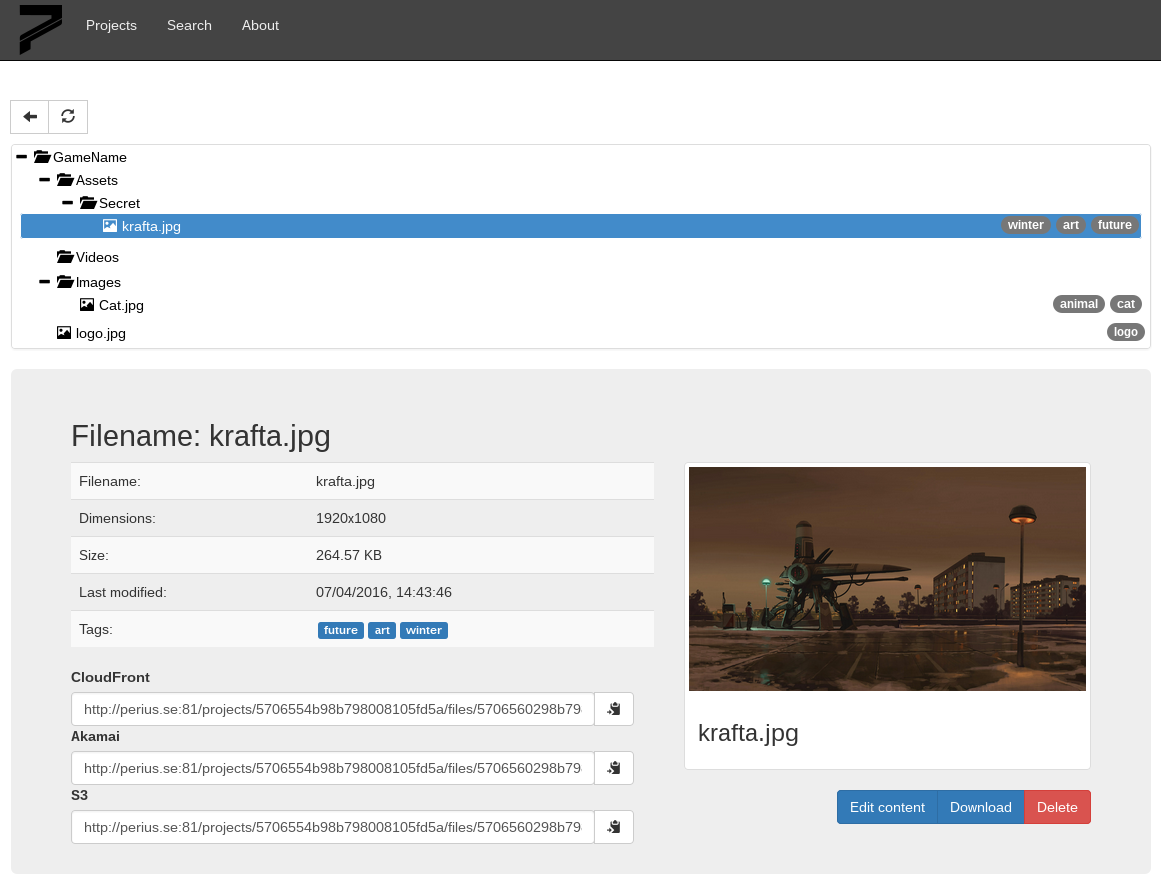
\includepdf[pages={1}]{front.pdf}
%\thispagestyle{empty}
%\newpage\null\thispagestyle{empty}\newpage

\pagenumbering{roman}
\setcounter{page}{1}

%\includepdf[pages={1}]{abstract.pdf}

%}}}
\begin{abstract}
This work presents a technique for implementing Copy-on-Write on top of an unaware persistent
storage. The system in this case is a security management system, but the technique and conclusions
drawn are general enough to be applicable to any system with vaguely similar consistency
requirements. The scalability of the storage system is tested and the technique is evaluated. The
technique is shown to be quite efficient (scalable to >6.000 simultaneous active users per node),
but a better solution is also suggested in the conclusion.\\

\keywords{CDN, Copy-on-Write, Eventual Consistency, MongoDB, Persistent Storage, Scalability, 
Software Security}
\end{abstract}

%{{{
\newpage\null\thispagestyle{empty}\newpage

\setcounter{tocdepth}{3}
\tableofcontents

\clearpage
\pagenumbering{arabic}
\setcounter{page}{1}

%}}}
\section{Introduction}
Developing large projects containing static content usually involves using a Content Distribution
Network to be able to scale to a larger user base. The commercial Content Distribution Networks are
usually fairly easy to use. The content that is to be used in a project is uploaded and then
distributed over the globe when a client is trying to access the content. For secret content this
can be a problem and an inconvenience, and that is what this thesis is about. 

When looking at the game industry, secret content could be anything from a picture related to a yet
unreleased game to an internal video only intended for employees. Some secret content needs to stay
secret and some content needs to get its security restraints changed during time. For example when a
game is in a closed alpha stage, the content should only be accessible by the people working on it.
But when that game later moves into an open beta phase (open for public), the content needs to be
publicly accessible. 

As large projects most often are divided into different dividable parts, a concept called containers
is introduced in this work. Containers can contain more containers and content, and when
modifying the security settings for a container it is applied recursively to all its content and
sub-containers.

This work examines a way of enforcing virtual access control on content and groups of content, in
the form of containers and snapshots to be able to handle the secrecy requirements easily. A system
was developed using the Copy-on-Write principle to improve scalability and make it a lighter
operation to take snapshots of parts of the system. 

The research question that this report tries to answer is how and whether it is practically 
feasible to use Copy-on-Write for a high-level system like the one that is implemented and how 
it can effect the system's scalability. 

\newpage
\section{Background}
This section gives the reader some background of the company where the thesis was written and
implementation was made. It also gives some brief explanations of the core concepts which are 
exerted throughout this work. 

\subsection{About Uprise}
Uprise (formerly known as ESN) is a company based in Uppsala, Sweden. It is an EA studio focusing on
creating great gaming experiences, which means that they are not focused on the actual gameplay, in
contrast to other EA studios like DICE. Historically Uprise has developed for example an
application called BattleLog, which is a companion for the BattleField game series. What Uprise is
currently working on is unfortunately classified.

\subsection{Prior Work}
The \textit{Prior Work} section goes through the related work that has already been made within the
area and which this thesis is based on.

\subsubsection{Copy-on-Write}
This work relies heavily on the Copy-on-Write principle, which was founded and used in the Mach
kernel~\cite{COPYONWRITE}, as it can be used to efficiently create snapshots and help solving
concurrency problems that otherwise can occur.

Copy-on-Write is used in for example virtual memory management systems~\cite{VIRTCOW}, snapshot
algorithms and as an optimisation technique for objects and types in several programming
languages\cite{LANGCOW}.

Its principle is that when processes or nodes share data in between each other, the data is not
copied until one of the processes makes changes to it. This is an optimisation as the processes do
not have to send or copy all of the related data that is in memory, rather they only have to send
pointers to the data. After many Copy-on-Writes a complex tree structure can be built up, but
optimisations can be done to simplify that structure~\cite{COPYONWRITE2}.

\subsubsection{Snapshots}
Several filesystems~\cite{BTRFS}\cite{ZFS} use snapshot techniques to make it possible for a user
or system to roll back the filesystems state, to a state that the filesystem had at the time of
snapshot creation. This can be useful for example when having a stable system and then doing a
system update, if the system does not respond well to the update the filesystem can be rolled
back to its previous stable state, provided that a snapshot was created before the update procedure.

This work has taken a lot inspiration from the way BTRFS~\cite{BTRFS} handles snapshots, which is
further explained in Section~\ref{sec:btrfs}.

\newpage
\subsection{Related Terminology}
In this section concepts and abbreviations, that are recurring throughout the paper, which the
reader needs to be familiar with are explained.

\subsubsection{Abbreviations}
\begin{description}

\item[CDN] \hfill \\
Content Distribution/Delivery Network - Replicates content to several servers, usually spread out
geographically. Once a request is made, the network serves content from the server closest to the
requester.

\item[GUID] \hfill \\
Global Unique Identifier - In distributed environments normal incremented identifiers can
not be used as there can be insertions on several nodes at the same time. A GUID is generated by a
function that makes it impossible or extremely unlikely that the same identifier will be generated
and used again.

\item[JPF] \hfill \\
Java Path Finder was developed by NASA and in 2005 they released it under an open source
license, which made more people contribute to the project. JPF is usually used for doing model
checking of concurrent programs to easily find for example race conditions and deadlocks.

\end{description}

\subsubsection{Terms}
\begin{description}
\item[Eventual Consistency] \hfill \\
Eventual consistency is an informal guarantee that defines how the consistency of stored data can
behave. In a system defined as using eventual consistency, access to stored data is not guaranteed
to return the result of the latest modification. At some point, if modifications to the stored data
stop, access to a data item will return the resulting data of the last modification of that
item.~\cite{EVENTUAL}. It is often used in the context of database systems.

The effect of the lack of a strong consistency requirement is that persistent storages, especially
distributed databases, can operate faster since there is no need for locks or transactions.  This
results in that operations on the same items can be made before earlier operations have propagated
to all the distributed nodes.

A system using eventual consistency can end up in a state where there is a conflict that needs to be
handled. If for example two concurrent operations performed on two different servers changes the
same data item, a conflict of how the resulting item should look like will occur when synchronising
these servers. To solve the conflict the system needs to have a defined set of rules to be able to
determine which operation that will take precedence, or how the concurrent operations are mixed,
which is usually called conflict or sibling resolution. %% Clock sync and check time as rule

\item[Perius] \hfill \\
Perius is the name of the implementation that was made during this project. It is an anagram of
Uprise and also a type of butterfly.

\item[Snapshot] \hfill \\
A snapshot is a way to record the full state of a system at a specific time. The term comes from
photography where a photo can be seen as the state of what the photo is of, at a certain time.
Snapshots should not be confused with a full copy of a system, or part of a system, as full copies
can be used as backups meanwhile snapshots are not very effective means of backup in the case of
data corruption. Snapshots are not effective against data corruption as snapshots usually still
refer to unchanged data that is still a part of the system~\cite{SNAPSHOT}.

\end{description}
\newpage
\section{Model} \label{sec:model}
This section describes how different operations can be expected to effect the data in the system.
The model for this work also shows how the data can only be accessed or modified by
authorized users and how the defined integrity of the data is always kept. 

There could also be another relevant part included in the model, to show that content can not be 
accessed by unauthorized viewers once the content is uploaded to a CDN. But as that should already 
have been thoroughly checked by the CDN providers this work can focus solely on the internal users 
and content in the management system. 

\subsection{Related work}
The model for this paper is based on the work that was done by Bell, D Elliott, LaPadula and 
Leonard J in their papers \textit{Secure computer systems: Mathematical foundations}~\cite{BLP1} 
and \textit{Secure computer systems: A mathematical model}~\cite{BLP2}. 
In these papers the foundation was laid for how to model computer systems to be able to analyse 
the security of them. Furthermore this paper was also inspired by Biba, \textit{Integrity 
considerations for secure computer systems}~\cite{BIBA}, where many of the points made by him was 
taken into consideration when inspecting that the integrity of the data was always sound.

\subsection{Approach}
As this work only presents an informal model of how the system is designed, it can not be regarded as
a proof for the actual implementation of the system to be flawless. The model should however give a 
strong idea of the soundness of the design of the system.

The Copy-on-Write principle is only used for files as all of the other objects in the system is
basically just metadata and not classed as important as the actual files themselves, from a data
integrity point of view.

\subsection{Sets and Elements of the Model}\label{sec:elements}
In this section we show the elements of the model, identify the different sets and explain how they
should be interpreted. This is done in the same way as in \textit{Secure Computer Systems: Mathematical
Foundations}~\cite{BLP1} by Bell \& LaPadula.

\begin{center}
    \begin{tabular}{ | l | l | l | p{5cm} |}
        \hline
        \textbf{Set} & \textbf{Elements} & \textbf{Semantics} \\ \hline
        C   & $c_0\dots c_n$                & Containers; folders in the virtual file system\\ \hline
        F   & $f_0\dots f_n$                & Files; files, images, videos\\ \hline
        M   & $m_0\dots m_n$                & Content; Metadata for files\\ \hline
        U   & $u_0\dots u_n$                & Users; registered users in the system\\ \hline
        A   & $A[u_0,c_0]\dots A[u_n, c_n]$ & Boolean Access matrix; access rights \\ \hline
    \end{tabular}
\end{center}

\begin{center}
    \begin{tabular}{ | l | l | l | p{5cm} |}
        \hline
        \textbf{Set} & \textbf{Relation} & \textbf{Type} \\ \hline
        \textbf{C} & $\textbf{C} \supseteq C \ni c$ & $\textbf{C}=P_{fin}(P_{fin}(C \cup M))$\\ \hline
        \textbf{M} & $\textbf{M} \supseteq M \ni m$ & $\textbf{M}=P_{fin}(M)$\\ \hline
        \textbf{F} & $\textbf{F} \supseteq F \ni f$ & $\textbf{F}=P_{fin}(F)$\\ \hline
    \end{tabular}
\end{center}

The bold notation (\textbf{C}, \textbf{M}, \textbf{F}) refers to the sets containing all possible
members of that type.

\begin{center}
    \begin{tabular}{ | l | l | p{5cm} |}
        \hline
        \textbf{Element} & \textbf{Type} \\ \hline
        c & $C \cup M$ \\ \hline
        m & $\{id: GUID, file: f\}$ \\ \hline
        f & File \\ \hline
    \end{tabular}
\end{center}


\begin{description}
\item[Container] \hfill \\
    A container is what would normally be called a folder in popular speech and in the terms of
    filesystems. A container can contain content objects and more containers, this recursive
    definition results in containers representing a virtual tree structure.

\item[File] \hfill \\
    A file is an actual file, in the same sense as in a file system. A file could be for example a
    video or image.

\item[Content] \hfill \\
    A content object contains a pointer to a file and metadata about that file. The pointer to the
    file within the object can change to a different file, but the content object still keeps the
    same metadata as before.

\item[User] \hfill \\
    A user is a registered user in the system.

\item[Access Matrix] \hfill \\
    The access matrix contains what containers that all the users in the system have access to. If
    A[u,c] is true in the access matrix, user \textit{u} has access to container \textit{c}.

\end{description}

\subsection{Access rights}
Access is only handled on containers and if a user has access to a container it also has access to
all of that containers children.
The \textit{A[u,c]} notation is symbolising an access token. If \textit{A[u,c]} is true in the 
access matrix \textit{A}, user \textit{u} has full access to the container object \textit{c} and its
children. If it is false or if the entry does not exist in the access matrix, the user \textit{u}
does not have any access rights for \textit{c}. 

\begin{equation}
    \begin{split}
        A[u,c] \Rightarrow & u \text{ can read } c \\
        A[u,c] \land \neg \text{ read-only(c) } \Rightarrow & u \text{ can write to } c \\
        A[u,c] \land \neg \text{ read-only(c) } \Rightarrow & u \text{ can delete } c \\
        A[u,c] \land f \in c \centernot\Rightarrow & u \text{ can delete } f 
    \end{split}
\end{equation}

\subsection{Data integrity}
A computer system or subsystem is defined as possessing the property of integrity if it behaves consistently
according to a defined standard. This implies that a subsystem possessing the property of integrity
does not guarantee an absolute behaviour of the system, but rather that it performs according to
what its creator intended ~\cite{BIBA}.
\\
The invariant for this model is the file. Which means that it should not be possible to
change a file though out the cycle of operation without creating a new file object with a new
identifier. This is to ensure that files can not lose their integrity by simultaneous
operations from different nodes or get mixed up when referred to from a content object. 

\subsection{Initial Assumptions}
To create an integrity model, some initial assumptions have to be made about what the correct
behaviour of the system is, which the model then can be shown to follow. In this work unintentional
behaviour as the result of data modification is the main concern, which could be used for sabotage
or simply be the effect unintentional unfortunate race conditions etc. 

\subsection{Integrity Threats}
According to Biba et. al~\cite{BIBA} one can consider two threat sources, namely subsystem external
and subsystem internal. The external sources could be another system calling the subsystem with
faulty data or trying to make inaccurate calls to program functions. Another external source could
also be somebody trying to tamper with the exposed functions of the program. Threats that are
internal could be a malicious part of the subsystem or simply an incorrect part of the subsystem,
which does not behave according to its specification.

In this work external threats are handled as threats that can occur from what has been exposed by
the API (See Section~\ref{sec:API}) and internal threats as incorrect implementation. As the server
and its system are assumed safe, malicious subsystems are not considered.

\subsection{Consequences of modification} \label{sec:conseq}

In this section the consequences, side effects and direct effects, of different operations are
stated in an informal mathematical manner, similar to how inference rules are composed. These rules
are what should be expected to be followed by the implementation in
Section~\ref{sec:implementation}. 

\begin{center}
    \begin{tabular}{ | l | l | l | p{5cm} |}
        \hline
        \textbf{Action} & \textbf{Semantics} \\ \hline
        u, read(m, f)    & User \textit{u} reads \textit{f} from \textit{m}\\ \hline
        u, create(m, c)  & User \textit{u} creates \textit{m} in \textit{c}\\ \hline
        u, update(m, f)  & User \textit{u} updates \textit{f} with \textit{m}\\ \hline
        u, delete(o)     & User \textit{u} deletes \textit{o}\\ \hline
        u, snapshot(o)   & User \textit{u} takes a snapshot of \textit{o} \\ \hline
    \end{tabular}
\end{center}

To describe a content object \textit{m} containing fileId \textit{f}, the following syntax is used:
$[fileId = f.id, \dots] \in M$, the same syntax is also applied to different types of objects
throughout the explanation of the model.

If the user is irrelevant for the rule described, it is left out from the action, for example u,
read(o) = read(o).

\vspace{2em}
\textbf{File Read}
\vspace{1em}
\begin{equation} \label{eq:fileread}
    \inferrule
    {(\textbf{*}) \\ C \ni c \ni m \\ A[u,c]} 
    {(C, F) \xrightarrow{u, read(m,f)} (C, F)}
\end{equation}
\vspace{1em}

A user \textit{u} with access rights to a parent container \textit{c} of content \textit{m}
can read a file \textit{f} in content \textit{m}.

These predicates are used in several places and are therefore named \textit{*}.

\vspace{2em}
\textbf{File Creation}
\vspace{1em}
\begin{equation} \label{eq:filecreate}
    \inferrule
    {C \ni c \\ A[u,c] \\ m \centernot \in c \\ \neg readOnly(c)} 
    {(C \cup \{c'\}, F) \xrightarrow{u, create(m,c)} (C \cup \{c \cup \{m\}\}, F \cup \{m.file\})}
\end{equation}
\vspace{1em}

A user \textit{u} with access rights to a non-readonly container \textit{c} can create a content
\textit{m}, containing a file \textit{f}, in container \textit{c}.

\vspace{2em}
\textbf{File Update}
\vspace{1em}
\begin{equation} \label{eq:fileupdate}
    \inferrule
    {\textbf{*} \\ c' = c \cup \{m'\} \\ m' = \{id = m.id, file = f'\} \\ \neg readOnly(c)} 
    {(C \cup \{c \cup \{m\}\} , F) \xrightarrow{u, update(m, f')} (C \cup \{c \cup \{m'\}\}, F
    \cup \{f'\}))}
\end{equation}
\vspace{1em}

If a user \textit{u} with access rights to a parent container \textit{c} (which is not read only) of
content \textit{m}, updates a file \textit{f} in content \textit{m}, the original file stays
intact as an effect of Copy-on-Write.

\vspace{2em}
\textbf{File Deletion}
\newline

Files can not be deleted by any user, however all the references to the file can
be deleted, see Consequence \ref{eq:delete}.

\vspace{2em}
\textbf{Content Update}
\vspace{1em}
\begin{equation} \label{eq:contentupdate}
    \inferrule
    {\textbf{*} \\ \neg readOnly(c)}
    {(C \cup \{c \cup \{m\}\}, F) \xrightarrow{u, update(m, m')} ((C \cup \{c \cup \{m'\}\}, F)}
\end{equation}
\vspace{1em}

If a user \textit{u} with access rights to a parent container \textit{c} of content \textit{m}
updates that content, the content is directly changed, without any Copy-on-Write.

\vspace{2em}
\textbf{Container Update}
\vspace{1em}
\begin{equation} \label{eq:containerupdate}
    \inferrule
    {\textbf{*} \\ \neg readOnly(c)}
    {(C \cup \{c\}, F) \xrightarrow{u, update(c, c')} (C \cup \{c'\}, F)}
\end{equation}
\vspace{1em}

If a user \textit{u} with access rights to a container \textit{c} updates that container, the
container is directly changed, without any Copy-on-Write.

\vspace{2em}
\textbf{Copy}
\vspace{1em}
\begin{equation} \label{eq:copy}
    \inferrule
    {\textbf{*} \\ m' = \{id = \text{"fresh"}, file = m.file\} \\ \neg readOnly(c)}
    {(C \cup \{c \cup \{m\}\}, F) \xrightarrow{u, create(c, m')} (C \cup \{c \cup \{m, m'\}\}, F)}
\end{equation}
\vspace{1em}

If a user \textit{u} with access rights to the parent (source and destination) container \textit{c}
of content \textit{m} copies that content, the new content \textit{m'} is not equal to the old
(because of its new ID), however they both contain the same file.

\vspace{2em}
\textbf{Content Deletion}
\vspace{1em}
\begin{equation} \label{eq:delete}
    \inferrule
    {\textbf{*} \\ \neg readOnly(c)}
    {(C \cup \{m\}, F) \xrightarrow{u, delete(m)} (C, F)}
\end{equation}
\vspace{1em}

If a user \textit{u} with access rights to a parent container \textit{c} of content \textit{m}
deletes that content, the file \textit{f} referred to in the content is not deleted.

\vspace{2em}
\textbf{Snapshot}
\vspace{1em}
\begin{equation} \label{eq:snapshot}
    \begin{split}
        [C', M'] := snapshot(tree) & \Implies \\
        \forall c \in tree, copy(c) \in & C' \\
        \forall m \in tree, copy(m) \in & M' \\
        \forall f \in tree, f \in & F
    \end{split}
\end{equation}

To explain the non-trivial snapshot operation it is first defined in \ref{eq:snapshot}. The snapshot
operation is performed upon a tree of objects and results in two new sets (C' and M'), one with
containers and one with content, the referred files remain the same as before the snapshot.

\vspace{2em}
\begin{equation} \label{eq:snapshot2}
    \inferrule
    {\textbf{*} \\ \neg readOnly(c)}
    {(C, F) \xrightarrow{[C', M'] := u, snapshot(c)} (C \cup C' \cup M', F)}
\end{equation}
If a user creates a snapshot of a container and the full container tree is re-created with new IDs,
but its content still refers to the same files.

\subsection{Interaction of Multiple Accesses} \label{sec:multiple_access}
As a result of consequence~\ref{eq:contentupdate} and~\ref{eq:containerupdate} in
Section~\ref{sec:conseq} there can be race conditions where the last write wins. This could be
solved by locks or transactions, but as updates are not based on each other, the trade-off for this
inconsistency to scalability and speed is intentional. However, as can also be seen in
consequence~\ref{eq:fileupdate}, if a file is removed from a content that file is not removed from
the set of files, even though its modification process is the last one to write to the content.
This is necessary as a file can be referenced from several content and the removal process can not
atomically ensure that the file is not referred to by another content. This results in a lot of
files in the system which are not referenced from anywhere. This can be solved by either making each
file keep track of how many times it is referred to and also make it possible to check this number
and delete the file in an atomic fashion. An easier approach would be to have a garbage collector
which locks parts of the system momentarily meanwhile it removes files which are not referenced. 

\par
There is also the chance to have content and containers that are not referenced from anywhere and
result in being garbage in the system. This could happen as a result of consequence~\ref{eq:delete}
in combination with any of the other consequences listed in Section~\ref{sec:conseq}. The basic idea
is that an entity is deleted meanwhile another is created or modified to have that entity as its
parent, thus creating a separate tree that can not be reached from the root node of the project.
These type of inconveniences should also be cleaned up by the garbage collector.

\subsection{JPF}
JPF was used to test the idea and state transitioning of the model. It is a very simplified
version of the real system that still contains all the important Copy-on-Write concepts and the 
assumptions that have been made in the model. This simplified version was then used to automatically
test for unwanted quirks. It is not a proof that the model works, but it is very exhaustive in its
testing.

\subsubsection{Entities}
\begin{figure}[H] 
    \centering{
        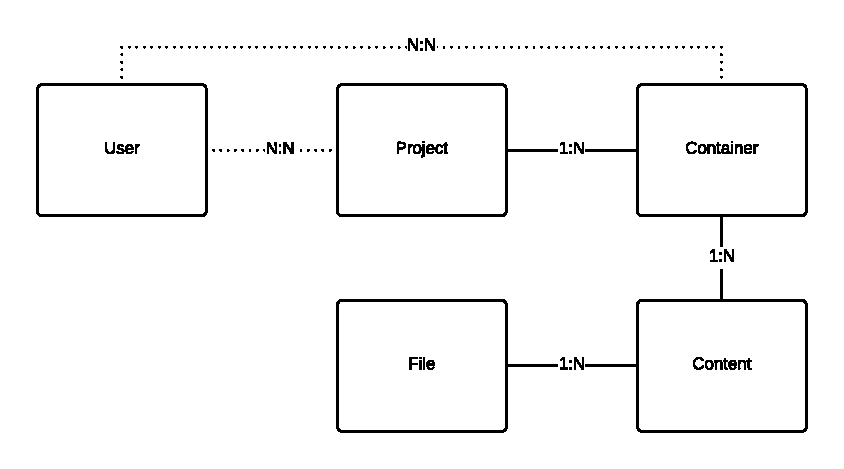
\includegraphics[scale=0.8]{relation.pdf}
    }
    \caption{High-Level Entity Relationships}
    \label{fig:relation}
\end{figure}

All the entities in Figure~\ref{fig:relation} is described in Section~\ref{sec:elements}, except for
projects, which is explained below. \\
\vspace{0.5em}

A \textbf{Project} is what is created to contain all content and containers related to a real project. Files
and metadata can only be changed within a project and the system can contain several projects 
that have their own virtual content and containers completely disjoint from the other projects.\\

\subsubsection{Execution}
Java Path Finder was used to show that the model and plan of how to build the system was sound. The
model was built in Java with the objective of being as reduced and simple as possible, without
loosing any of the cases that needed to be covered by the model checker. As the users are mainly
going to be handled by external systems they were not included in the model.

Each collection in the persistent storage was emulated by using the built-in ConcurrentHashMap type.
Each client was represented by a thread and each action taken by the client was randomised. The ID
hash function which MongoDB is using for each entity was imported from the mongo-java-driver-2.13.3
and each object had its own ID, generated in the same fashion as the real implementation. The ID's
are randomly generated by the ObjectId class to minimise or completely avoid collisions.
Furthermore no locking or transactions were used and the threads were running fully concurrently and
without any sleep statements. 

ConcurrentHashMap had to be used in instead of the normal HashMap, as the normal HashMaps can not 
be iterated over concurrently.

JPF checked each permutation of states, to a certain depth, that the threads can end up in and the 
result of the run can be seen in Listing~\ref{JPFRESULT}.

\begin{minipage}{\linewidth}
\begin{lstlisting}[label=JPFRESULT,caption=Results of JPF run]%,float,floatplacement=H]
elapsed time:       14:26:53
states:             new=160853259,
                    visited=451102505,
                    backtracked=611955764,
                    end=21640
search:             maxDepth=380,
                    constraints=0
choice generators:  thread=160853255 
                    (signal=0,
                    lock=3603938,
                    sharedRef=146989208,
                    threadApi=3,
                    reschedule=10260106), 
                    data=0

heap:               new=676056850,
                    released=435060996,
                    maxLive=655,
                    gcCycles=523950061

instructions:       11917045758
max memory:         6256MB
loaded code:        classes=111,
                    methods=2179
\end{lstlisting}
\end{minipage}

\subsection{Findings}
This section summarises the findings from the work on the model. 

\subsubsection{Garbage Collection}
For the system to reach a clean state and the decided eventual consistency~\cite{KLINGSBO}, garbage
collection will be needed. As of the conclusion in Section~\ref{sec:multiple_access} from Section
~\ref{sec:conseq} there will be objects in the system that are unreferenced and can not be reached
and should therefore be cleaned up for them not to cause negative performance effects on the system.

\subsubsection{Conflict Resolution} \label{sec:conflict_res}
If the persistent storage would be distributed, the different database nodes would have to have rules
set up for conflict resolution as this model does not consider what to do if the same metadata is
modified on the nodes before they have time to synchronise. The easiest way to handle this is to
have the clocks on the nodes synchronised and timestamp each change and when synchronising the nodes
only consider the newest data if there is a conflict. This will have the same result as concurrent
modification with a single database node with this model, namely last write
wins~\cite{LASTWRITEWINS}.

\subsubsection{JPF Results}
Although the JPF model checking results did not return any errors or showed any possible misbehaviours
of the model, it should not be considered proven. The results however strongly indicate that there are no
major flaws in it. But as the model will be more complicated once fully implemented as an application
there might be flaws in the implementation details. 

\newpage 
\section{Implementation} \label{sec:implementation} 
This chapter deals with the second part of this work, namely the implementation of the Perius
system. The implementation is based on the model described in Section~\ref{sec:model}. As this work
is not intended as an instructions manual, more information about how to deploy and use Perius can
be found on \url{http://perius.se}. This chapter's focus is instead on how the decisions for the
implementation were made, how well the system would scale and the resulting security implications.

\subsection{Background} \label{sec:background}
Section~\ref{sec:background} explains the problem at hand, in relation to the system currently 
used.

\subsubsection{The current system} \label{sec:current_system}
Today a system called Battlebinary~\cite{BATTLEBINARY} is used for managing and uploading files,
mostly images, to content delivery networks. The current system does not make use of the
security features that the CDNs are offering, instead it uses a form of security by obscurity. When
a file is uploaded to a CDN it is open for the public, but its filename is composed out of its
original filename concatenated with a part of the MD5 hash of the content of the file, which makes
it an extremely hard process to access the file on the CDN without access to the original file or a
reference to the URI.

In the current system you can only upload a file once as there will be a collision in the upload
otherwise, as the old and the new file will have the same MD5 hash, which is by design as duplicate
content just wastes space on the CDN. The problem with this is that the current interface does not
handle it very well as one file can not be shown or uploaded in two different places in 
Battlebinary's virtual filesystem.

\subsubsection{Problem description}
The current system does not offer proper security measurements, is lacking a lot of features that
are needed and does not scale very well, hence a new system are to be developed. This work is about
examining a way of implementing Copy-on-Write in a high-level system like this, which should solve
the scalability problem and make it possible to implement wanted features like snapshots, cloning
and concurrent modifications of content.

\begin{figure}[H] 
    \centering
    \renewcommand{\arraystretch}{1.3}
    \begin{tabular}{|r|l|}
        \hline
        Application &
        \begin{tabular}{|r|l|}
            \hline
            Perius Front-end\\
            Perius Back-end\\
            \hline
        \end{tabular}\\
        Persistent Storage & MongoDB \\ \cline{2-2}
        Filesystem & Ext4 \\ \cline{2-2}
        OS & Arch Linux \\
        \hline \hline
        Hardware & \\
        \hline
    \end{tabular}
    \renewcommand{\arraystretch}{1.0}
    \caption{Software Stack}
    \label{fig:stack}
\end{figure}

To clarify what is meant by Perius being high-level software the stack in Figure~\ref{fig:stack} can
be examined. Theoretically the Copy-on-Write features could be implemented in any of the separate
parts of the stack to support the features that Perius has to achieve, in this work only the second
highest layer is considered, the Perius back-end.

\subsection{Architecture and Technologies used} \label{sec:tech}
This section introduces the different technologies used in the implementation. The section also
contains motivations and explanations why certain technologies were chosen and briefly outlines the
software architecture. 

\begin{figure}[H] 
    \centering{
        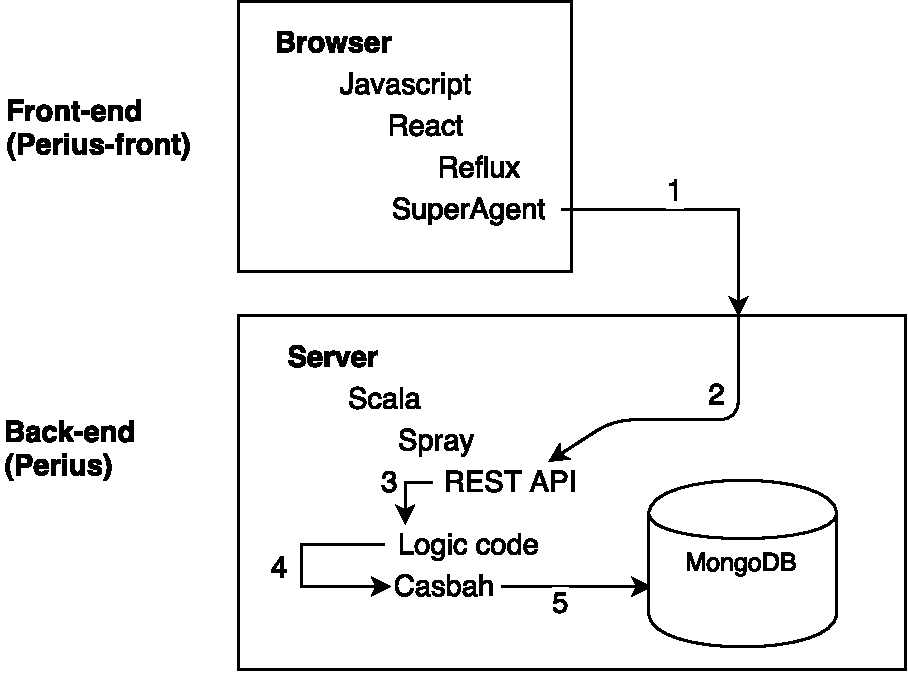
\includegraphics[scale=0.8]{techstack.pdf}
    }
    \caption{Technology Stack}
    \label{fig:tech_stack}
\end{figure}
Figure~\ref{fig:tech_stack} shows how the different technologies used are related. In the Figure, 
the technologies that are indented are built on top of its parent. The arrows that can be seen is
the flow of data after a request from the front-end has been made. The arrows are unidirectional,
but the response follows the same path back to the requester.

\begin{description}

\item[Javascript]
is a programming language mainly focussed on running code in web browsers~\cite{JAVASCRIPT}. In this
implementation the ECMAScript 6 (ES6) language specification is used, which adds a lot of syntactic
sugar compared to what usually is called normal JavaScript. An example of such syntactic sugar is
lambda expressions. React and Reflux are both built with JavaScript in mind and is used on top of
JavaScript is this implementation, as can be seen in Figure~\ref{fig:tech_stack}. 

\item[SuperAgent]
is a small HTTP request library which can be used from client-side Javascript or as a node.js
module~\cite{SUPERAGENT}. It is used to form the requests to the REST API from the front-end, which
can be seen in Figure~\ref{fig:tech_stack} (Arrow 1 and 2).

\item[React]
is a JavaScript library for building user interfaces. React uses both its own virtual DOM and
the browser's normal DOM, this makes it able to efficiently update dynamic web pages after a change
of state through comparing the old virtual DOM with the resulting virtual DOM after the state change
and then only update the browser's DOM according to the delta between the virtual DOMs~\cite{REACT}.
React can be seen as the system for handling views in front-ends implementing a MVC-like
(Model-View-Controller) architecture. In this work React is used as a part of building the
front-end.

\item[Reflux] 
is an idea and a simple library of how to structure your application~\cite{REFLUX}. It features a
unidirectional dataflow (see Figure~\ref{fig:reflux}) which makes it more suitable, than for example
Flux~\cite{FLUX}, when using a functional reactive programming style. Reflux is used together with
React for this implementation to define a structure of the flow of data and state changes.

\begin{figure}[H] 
    \centering
    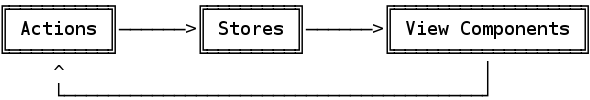
\includegraphics[scale=0.4]{reflux.png}
    \caption{Reflux unidirectional dataflow}
    \label{fig:reflux}
\end{figure}

\item[Scala]
is a multi-paradigm programming language. It most commonly runs on the JVM and unlike Java it
supports most functional programming features at the same time as it supports object-oriented
programming~\cite{SCALA}. Scala is used to program the back-end and the Spray toolkit is used with
it to simplify the API.

\item[REST]
stands for representational state transfer, it is an architectural idea for writing stateless
services. These services usually use URIs to identify specific resources and HTTP to modify or query
these resources~\cite{REST}. 

In this work a RESTful API was implemented and used for back-end $\Iff$ front-end
communication, which can be seen in Figure~\ref{fig:tech_stack} (Arrow 1 and 2).

REST was chosen as all operations that needs to be performed can be defined as basic CRUD operations
and because the BSON format which is used in MongoDB is almost identical ~\cite{BSON} to the
standardised JSON format which is usually used by RESTful services~\cite{JSON}. 

\hfill \\
\textbf{REST Endpoints} \label{sec:API} \hfill \\
For the front-end to communicate with the back-end, a RESTful service is implemented.
The following endpoints were configured:

\begin{itemize}
  \item projects
      \subitem GET - list all projects
      \subitem POST - create new project
  \item projects/\{id\}
      \subitem GET - get specific project
      \subitem PUT - update existing project
      \subitem DELETE - delete existing project
  \item projects/\{id\}/content
      \subitem POST - create new content in a specific project 
  \item projects/\{id\}/content/\{id\}
      \subitem GET - get specific content in a specific project
      \subitem PUT - update existing content in a specific project
      \subitem DELETE - delete existing content in a specific project

  \item projects/\{id\}/snapshots
      \subitem POST - create new snapshot in a specific project 

  \item projects/\{id\}/containers
      \subitem POST - create new container in a specific project 
  \item projects/\{id\}/containers/\{id\}
      \subitem GET - get specific container in a specific project
      \subitem PUT - update existing container
      \subitem DELETE - delete existing container
\end{itemize}

As can be seen several expected endpoints are missing, this is intentional as the operations missing
can be performed in a more efficient way. Such endpoint is for example \textit{GET 
projects/\{id\}/containers} as all containers exist in \textit{GET projects/\{id\}} and the interface
should present a file structure where both content and containers are shown.

% \hfill \\ %\label{sec:spray}
\item[Spray]~\cite{CASBAH} % Spray in casbah book
is an open-source toolkit written in Scala and for Scala. It is used to make it easier to build
REST/HTTP APIs and those abilities is what it is used in the implementation.

\item[MongoDB]% \hfill \\ %\label{sec:spray}
is a document-oriented database, which means that it does not have the concept of rows as
normal relational databases has. Instead each entity in the database is stored as a document which
is not fixed to a predefined table structure~\cite{MONGODB}. MongoDB lacks the support for joins to
improve its possibility to scale, which can be a big downside to some applications containing the
need for such logic. MongoDB is used as a persistent storage for the back-end to store all the
projects and nodes in the tree structures and also the files uploaded to the system. The Scala logic
code uses a layer called Casbah~\cite{CASBAH} to interface with MongoDB, which can be seen in
Figure~\ref{fig:tech_stack} (Arrow 4 and 5).

\par MongoDB was chosen as the persistent storage because of its quick lookups and because of its
internal storage format called BSON, which is very similar to JSON which the API is using. As the
formats are similar, the process of marshalling and unmarshalling becomes quite easy between the
core code, MongoDB instance and REST interface.  The second reason was that if the system needs to
scale in the future it is very easy to distribute MongoDB and, if needed, the system can easily be
migrated to Reactive Mongo. Reactive Mongo is an asynchronous and non-blocking driver for MongoDB
and can therefore make the system scale even further~\cite{REACTIVEMONGO}.

\par All files are also stored directly in MongoDB with the help of GridFS. GridFS chunks the files 
according to the size limit of MongoDB objects, which is currently 4MB. The advantage of this is 
that backups of the Perius system is easily done through a database backup, no separate files 
needs to be backed up. Another advantage that is given by this is that you can retrieve specific 
ranges of a file, although that advantage is not needed in the Perius implementation. For
scalability this could be used to retrieve different parts of a file from different servers, 
normal load balancing would probably work better in a system like Perius where no extremely large 
files are expected to be stored. 

\par The disadvantage of using the GridFS approach is that when using a non-distributed database 
it is slower to read and write to the database than reading or writing directly to a filesystem. 
Another disadvantage is that to access the files it is needed to go through the database layer 
in some way, instead of accessing the filesystem directly.


\end{description}
\subsection{Methods for determining\\implementation details}
This chapter introduces the different methods used to determine how the new system should be
implemented, which persistent storage it should use and how the estimation of long-term scaling 
was done.
\\
\par As this work was not mainly about the system architecture, but rather about evaluating the
effects of using Copy-on-Write, the decisions taken for the different technologies used were simply
made from what the author was comfortable with and knew would have little impact on the evaluation. 
With that said there are no comparisons of for example different databases, protocols or API
solutions in this paper.

\par The long-term scaling was done by load testing the back-end with Wrk and Apache Bench. With
the help of these tools, the computationally expensive operations could be found and it could be
determined what the upper bound for how many active users the system could handle on a node with
similar hardware specifications.

\par A low timeout was set to make sure that the system could handle operations faster than they
queued up. This was to be certain that the system could sustain the number of active users during a
longer time frame without having a queue which grows beyond a manageable size.

\subsection{Copy-on-Write} \label{sec:copy-on-write}
This section is about how Copy-on-Write was used in Perius and how its implementation of it differs
from other systems that incorporate Copy-on-Write.

\subsubsection{Snapshot Functionality}
The Copy-on-Write concept is not only well-suited for consistency requirements, it is also works 
well for creating snapshots.

To efficiently create snapshots of a system, Copy-on-Write can be used to make it possible to create
snapshots in O(1)\cite{BTRFS}. This is due to the fact that to create a snapshot in a system using
Copy-on-Write you only need to reference the current nodes in the tree and make sure that they are
not removed, see Figure~\ref{fig:btrfs_tree}.

\subsubsection{Full Copy}
Full Copy or Deep Copy, as opposed to Copy-on-Write, is a copy where everything is copied directly
and not only when an object is changed. This is easier to implement but is in most cases more
inefficient as more disk space will have to be used and if used with for example certain tree 
structures the part of the tree that needs to be copied will have to be traversed. 

\subsubsection{Examples of Copy-on-Write system implementations}
\subsubsubsection{BTRFS} \label{sec:btrfs}
Btrfs is a B-tree file system for Linux which makes use of Copy-on-Write to make it able to do
efficient writeable snapshots and clones. It also supports cloning of subtrees without having to
actually copy the whole subtree, this is due to the Copy-on-Write effect. As several nodes in the
tree can refer to the same node each node keeps track of how many parents it has by a reference
counter so that the node can be deallocated once the node does not have any parents any more. The
reference counter is not stored in the nodes themselves but rather in a separate data structure so
that a node's counter can be modified without modifying the node itself and therefore eludes the
Copy-on-Write that would have to occur.

\begin{figure}[H] 
    \centering{
        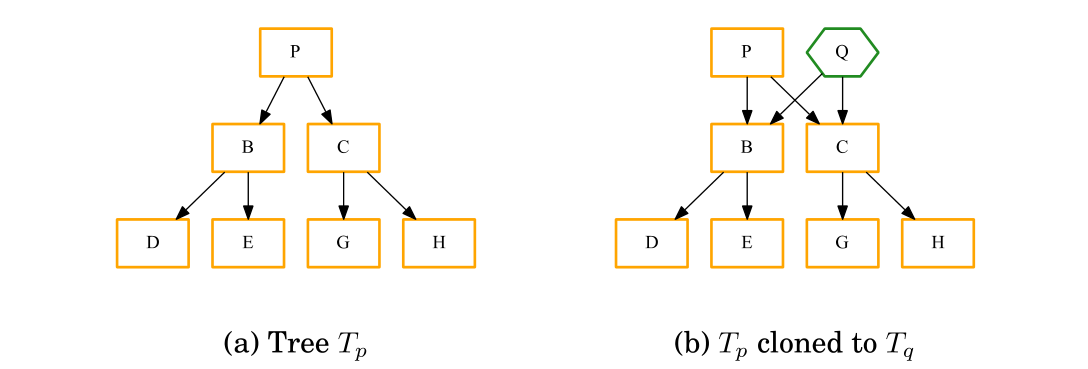
\includegraphics[scale=0.4]{newtree.png}
    }
    \caption{Cloning mechanism of Btrfs~\cite{BTRFS}}
    \label{fig:btrfs_tree}
\end{figure}

\subsubsubsection{Mach kernel}
In the mid 80's when the development of the Mach kernel started, there was problems with that
physically copying memory was too slow. To minimise the copying of memory, Copy-on-Write was
implemented. It was implemented so that virtual copy operations could be done and so that tasks
could share read-write memory~\cite{MACH}.

\subsubsection{Perius}
As the persistent storage, used in this implementation (Section~\ref{sec:tech}), does
not implement transactions or locks a lot of different problems can occur when several clients are
working on the same data set at the same time. Such problems could be race conditions or determining
the happened-before relation~\cite{LAMPORT}. In this work the race condition problem is solved by 
implementing Copy-on-Write on data with high consistency requirements. The happened-before relation
is not fully solved, but suggestions of how to solve it is given in Section~\ref{sec:conflict_res}.

\begin{figure}[H] 
    \centering
    \begin{subfigure}{.3\textwidth}
        \centering
        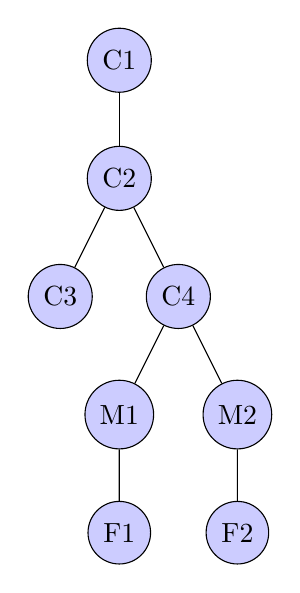
\begin{tikzpicture}[nodes={draw, circle, fill=blue!20}, -]
            \node{C1}
                child{node{C2} 
                    child{node{C3}} 
                    child{node{C4} 
                        child{node{M1} child{node{F1}}}
                        child{node{M2} child{node{F2}}}
                    }
                };
        \end{tikzpicture}
        \caption{Original Tree}
        \label{fig:orignal_tree}
    \end{subfigure}\qquad
    \begin{subfigure}{.4\textwidth}
        \centering
        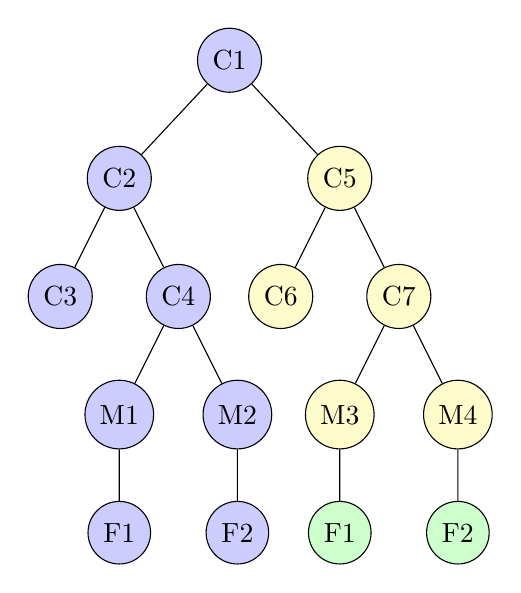
\begin{tikzpicture}[nodes={draw, circle, fill=blue!20}, -, level 1/.style={sibling
             distance=28mm}, level 2/.style={sibling distance=15mm}]
             \node{C1}
                 child{node{C2} 
                     child{node{C3}} 
                     child{node{C4} 
                         child{node{M1} child{node{F1}}}
                         child{node{M2} child{node{F2}}}
                     }
                 }
                 child{node[fill=yellow!20]{C5} 
                     child{node[fill=yellow!20]{C6}} 
                     child{node[fill=yellow!20]{C7} 
                         child{node[fill=yellow!20]{M3} child{node[fill=green!20]{F1}}}
                         child{node[fill=yellow!20]{M4} child{node[fill=green!20]{F2}}}
                     }
                 };
         \end{tikzpicture}
         \caption{Tree with C2 Snapshot}
         \label{fig:snapshot_tree}
    \end{subfigure}
    \caption{Snapshot Explanation\\ C - Container, M - Content, F - File}
    \label{fig:snapshot_expl}
\end{figure}

In Perius, snapshots and clones are not taken in the fashion which Btrfs uses, which can be seen in
Figure~\ref{fig:btrfs_tree}. As Perius does not have the tree structure pre-built and each node is
instead stored in a flat storage space, such operation would be too computationally expensive as
trees would have to be merged when collisions occur, due to the non-blocking nature of the
application. Instead this implementation makes a full copy of the metadata of the tree, but still
refers to the same binary files until the metadata is changed to point to another file.

Figure~\ref{fig:snapshot_expl} shows how a snapshot is performed on C2 and stored in C1, and how the
resulting tree would look like. In Figure~\ref{fig:snapshot_tree} all of the yellow nodes are copies
of metadata that were in the left tree, for example C5 and C2 contain the same data (except for
their newly generated IDs). The green nodes refer to files that have not been copied but are still
referenced in the copied metadata, this is due to the fact that a snapshot is not a write to the
files and they are therefore not copied but remain intact.

\subsection{Resulting system}
The \textit{Resulting System} section explains what the implementation looks like and how its
different operations work, in the terms of efficiency. 

\subsubsection{Perius}
Perius is the implementation that was done to solve the problem at hand at Uprise. Perius has a
back-end written in Scala and a front-end written in Javascript (ES6), but they are both
interchangeable. The back-end has a REST API running, which is how the front-end communicates with
the back-end.

\begin{figure}[H] 
    \centering{
        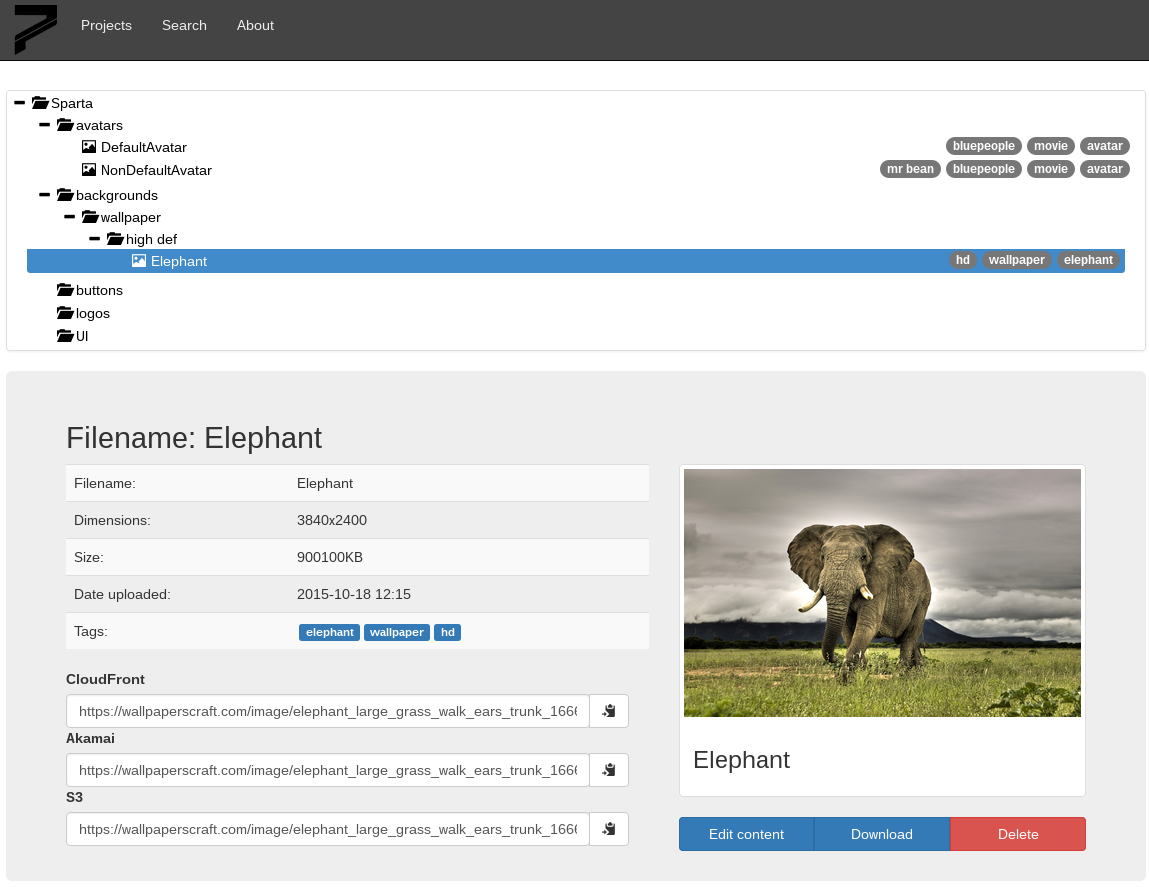
\includegraphics[scale=0.35]{frontend.png}
    }
    \caption{Front-end~\cite{BTRFS}}
    \label{fig:frontend}
\end{figure}

The service features a virtual file structure over the assets and metadata that have been stored,
as can be seen in Figure~\ref{fig:frontend}. It also features snapshots, security management of
whole containers as well as individual files, audit and auth logging, multiple separate project 
and a design which allows for an interchangeable persistent storage.

The front-end is written in ES6 with React and Reflux, and the styling is done with the help of
Bootstrap.

\subsubsection{Entities of the Implementation}
This section explains the different types of entities, and their interaction, that are handled by
Perius. They are explained similarly to how they are explained for the model in
Section~\ref{sec:elements}, but with more implementation specific details.

\begin{description}
\item[Content] \hfill \\
Content is metadata about a file and is stored in a container, it is a form of virtual file.  The
content can refer to for example an image, video or binary blob.\\

\item[Project] \hfill \\
A project is what is created to contain all content and containers related to a real project. Files
and metadata can only be changed within a project and the system can contain several projects 
that have their virtual content and containers completely disjoint. Each project is handled as a
separate database in MongoDB.\\

\item[Container] \hfill \\
A container is a virtual folder within a project which can contain content and other containers.\\

\item[Snapshot] \hfill \\
A snapshot is a read-only container from the state which the container was in when the snapshot
was created.  A snapshot can not be updated and can only be deleted from the root of the snapshot.
Snapshots are by default stored as siblings to the container which they were made from, but they can
be contained by any container.\\

\item[File] \hfill \\
A file refers to an actual physical file. Files are stored in the database to make backup,
deployment and migration easier.\\

\item[User] \hfill \\
A user is the structure that handles people who have been granted access to the system. Access to
the system is handled by a separate service, like LDAP.\\

\end{description}
\subsubsection{Runtime Complexity of Operations} \label{sec:run_time}
The runtime complexities of the operations in this section are quite intuitive, that is why they 
are only explained, and not proven to fulfil the complexities which are claimed. 
%To prove them, methods like the master theorem~\cite{ALGORITHMS} or \dots could be used.

\begin{figure}[H] 
    \centering{
         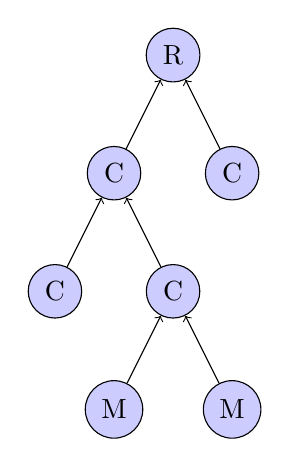
\begin{tikzpicture}[nodes={draw, circle, fill=blue!20}, <-]
             \node{R}
             child{node{C} child{node{C}} child{node{C} child{node{M}} child{node{M}}}}
             child{node{C}};
         \end{tikzpicture}
    }
    \caption{Project Tree\\R - RootContainer, C - Container, M - Content}
    \label{fig:project_tree}
\end{figure}

In the user interface the stored data is always represented and worked on as a tree, or a forest if
all projects are considered. For a very small project that tree could look like the example in
Figure~\ref{fig:project_tree}. This is however not what the actual storage of the data looks like.

\begin{figure}[H] 
    \centering
    \renewcommand{\arraystretch}{1.3}
    \begin{tabular}{|r|c|l|}
        \hline
        \textbf{Type} & \textbf{ID} & \textbf{Parent ID} \\
        \hline
        RootContainer & 1 & 1 \\
        Container     & 2 & 1 \\
        Container     & 3 & 1 \\
        Container     & 4 & 2 \\
        Container     & 5 & 2 \\
        Content       & 6 & 5 \\
        Content       & 7 & 5 \\
        \hline
    \end{tabular}
    \renewcommand{\arraystretch}{1.0}
    \caption{Simplified Representation of the Actual Storage}
    \label{fig:storage}
\end{figure}

The actual storage of the data is represented by documents in a flat document storage, which is in
this case MongoDB. A very simplified version of how the data is stored can be seen in
Figure~\ref{fig:storage}, however in reality it is not quite so table-like. One important point that
differs in the example and in the actual storage is that GUIDs are used for identifiers and not
incremented numbers, as that would not work in distributed environments. 

The data is not stored as a tree (see Example~\ref{fig:storage}), but rather as separate documents 
loosely referring to each other. How the different operations perform their actions and what 
implications these actions have on the operations run-time complexities are not obvious and that 
is what is discussed in this section.\\

\par \textbf{GET single entity} \\
When the back-end is handed a GET request it looks at what type of entity that is requested and
returns the document with the correct ID from the corresponding collection. As the collections are
hash indexed on ID this operation can be made in constant time, O(1) and thus $\theta(1)$. \\

\par \textbf{GET project tree} \\
When requesting a project the full project tree with all entities except files has to be built as
the entities not are stored as a tree in MongoDB. The tree is built layer by layer by fetching
content with the same parent ID, starting from the root of the project. Parent ID's are also indexed
by a hash index which makes it possible to get all nodes with the same parent ID in constant time.
This has to be done for every level with a different parent in the tree which makes the upper bound
O(n) if all of the subtrees only have one node each. The tight bound can not be calculated as the
trees balance is not determined by an algorithm but rather by a user, but from observation one could
argue that the trees usually have several nodes for each parent node in the tree, which then would
give a logarithmic tight bound, $\theta(log(n))$.\\

\par \textbf{POST/Create entity} \\
Creating a new entity in the system is a constant time operation for containers and content as they
only have to be inserted as new documents in MongoDB, which is a O(1)
operation~\cite{MONGOPERFORMANCE}. Even though the insertion itself has constant run-time the index
needs to be updated or sometimes even rebuilt, which can slow down the time before the document is
accessible in constant time. When inserting files they need to be chunked into pieces and inserted
into GridFS, this results in n/s insertions where n is the size of the file and s is the chunk size.
The insertion of files can then be regarded as O(n) if the size of the file is regarded, but if n is
regarded as the number of files in the system the upper bound is constant as the insertion for files
is made in the same way as for other documents.\\

\par \textbf{Snapshot creation} \\
In the creation of a snapshot all metadata in the tree that the snapshot is taken of is duplicated,
meanwhile the files remain the same, this results in n insertions where n is the number of
containers and content entities in the subtree. A snapshot insertions runtime is therefore
$\theta(n)$ and O(n). \\

\par \textbf{Delete entity} \\
Deleting an entity is a constant time operation when that entity does not have any children. When
the entity has children all those children has to be deleted too which will be done in the same
manner as the project tree is built and therefore results in the same runtime, O(n) as an upper
bound, where n is the number of entities in the subtree.\\

\par \textbf{PUT/Update entity} \\
The update operation in MongoDB completely replaces a document with another in regards to their
unique identifier. This could be seen as a deletion of the old document and an insertion of a new
one, but with the same ID, which makes it unnecessary to update the index for the unique ID. Other 
indices might have to be updated though, if for example the parent of the document is changed. 
As both deletion and insertion are constant time operations, update is also O(1).\\

\subsubsection{Copy-on-Write}
This implementation is far from as efficient as the other Copy-on-Write systems described in
Section~\ref{sec:copy-on-write} in most aspects, but more efficient in some. As the implementation
is built upon MongoDB as persistent storage and not a pure tree structure, single nodes can be
fetched in O(1) but when querying for subtrees they need to be built first, which arguable (See
Section~\ref{sec:run_time}) takes $\theta(log(n))$, where n is the number of nodes in the subtree. 

%\subsubsection{Persistent storage} \label{sec:persistent_storage}
\newpage
\subsection{Load Testing} \label{sec:load_testing}
Wrk and Apache Bench was used to load test the back-end. Wrk is a multi-threaded benchmarking tool
for HTTP which can create large loads and Apache Bench has similar capabilities, but is better
suited for file uploads than Wrk. The testing was done locally on a virtual server having 6 CPU
cores and 48GB of RAM. The results that will be analysed are the throughput of each request
performed without breaking the set timeout of the server, as that will give a fair judgement of how
well the system can perform.

\subsubsection{GET requests} \label{sec:GET_REQUESTS}
To be able to determine what the bottleneck of the back-end is, three different types of \textit{GET
requests} are performed. Most responses are JSON structures, except for the ones in
Listing~\ref{OKREQUEST} and Listing~\ref{STATICREQUEST}, which can be seen in the Response data part
of the listings.\\

The typical requests performed with Wrk in this work will look similar to this:
\begin{lstlisting}[frame=single]
wrk -t100 -c100 -d10s http://perius:8000/ok
\end{lstlisting}
where -t100 means that it uses 100 threads, -c100 that it emulates 100 clients requesting over and
over and -d100s is the amount of time that the load test will run, in this case 100 seconds.

\begin{minipage}{\linewidth-1cm}
\begin{lstlisting}[label=OKREQUEST,caption=Result of OK requests]
wrk -t100 -c100 -d10s http://perius:8000/ok

Running 2m test @ http://perius:8000/ok
  100 threads and 100 connections
  Thread Stats   Avg      Stdev     Max   +/- Stdev
    Latency     1.22ms    3.20ms 166.78ms   97.75%
    Req/Sec     1.04k   152.50     2.25k    79.18%
  10345746 requests in 1.67m, 1.69GB read
Requests/sec: 103353.85
Transfer/sec:     17.25MB

Response data:
200 OK
\end{lstlisting}
\end{minipage}

\par
The first request (Listing~\ref{OKREQUEST}) tries to maximise the number of requests that spray-can
(HTTP server) can handle with the given specifications and therefore the server just returns 200
(OK).

\begin{custommargins}{0cm}{-2cm}
\begin{minipage}{\linewidth-1cm}
\begin{lstlisting}[label=DBREQUEST,caption=Result of MongoDB requests]
wrk -t100 -c100 -d10s http://perius:8000/projects

Running 2m test @ http://perius:8000/projects
  100 threads and 100 connections
  Thread Stats   Avg      Stdev     Max   +/- Stdev
    Latency    14.52ms   13.34ms 375.51ms   99.31%
    Req/Sec    72.85      6.91   232.00     60.20%
  726351 requests in 1.67m, 196.03MB read
Requests/sec:   7256.38
Transfer/sec:      1.96MB

Response data:
[{
  "id": "565cdae1898b798008105fd47",
  "name": Test Project,
  "readOnly": false,
  "lastModified": 1456320024643
}]
\end{lstlisting}
\end{minipage}
\end{custommargins}

\par
The second request (Listing~\ref{DBREQUEST}) performs the simplest API call which involves getting
all currently stored projects from the MongoDB instance. This request does not yield any extra
computation in the back-end, apart from converting the MongoDB format to the API's JSON result
format.

\newpage
\begin{custommargins}{0cm}{-2cm}
\begin{minipage}{\linewidth-1cm}
\begin{lstlisting}[label=STATICREQUEST,caption=Result of static text requests]
wrk -t100 -c100 -d10s http://perius:8000/static

Running 2m test @ http://perius:8000/static
  100 threads and 100 connections
  Thread Stats   Avg      Stdev     Max   +/- Stdev
    Latency     6.42ms   28.99ms 290.37ms   96.26%
    Req/Sec     0.94k   203.30     2.00k    83.83%
  9199737 requests in 1.67m, 2.19GB read
Requests/sec:  91902.48
Transfer/sec:     22.44MB

Response data:
Static test data for WRK not involving MongoDB 
or filesystem access. 
Lorem ipsum dolor sit amet, consectetur adipiscing elit.
\end{lstlisting}
\end{minipage}
\end{custommargins}

\par
As the second request (Listing~\ref{DBREQUEST}) involves the server answering with some payload that
is generated from the persistent storage, the third request (Listing~\ref{STATICREQUEST}) is simply
the same amount of static payload as the second request but without involving any connections to
MongoDB. This was done to be able to estimate what impact the round trip time to MongoDB and the
conversions to the response format had on the throughput.

\begin{minipage}{\linewidth-1cm}
\begin{lstlisting}[label=TREEREQUEST,caption=Result of project tree requests]
wrk -t10 -c10 -d10s http://perius:8000/projects/56...
 
Running 10s test @ http://perius:8000/projects/56...
  10 threads and 10 connections
  Thread Stats   Avg      Stdev     Max   +/- Stdev
    Latency   247.54ms   21.64ms 323.78ms   96.76%
    Req/Sec     3.80      1.22    20.00     99.00%
  401 requests in 10.07s, 9.67MB read
Requests/sec:     39.82
Transfer/sec:      0.96MB

Response data:
{
  "parent": "",
  "name": "Test Project",
  "readOnly": false,
  "lastModified": 1456320024643,
  "id": "56cdae1898b798008105fd47",
  "containers": [{
    "parent": "56cdae1898b798008105fd47",
    "name": "Upload stuff",
    "readOnly": false,
    "lastModified": 0,
    "id": "56cdae2298b798008105fd48",
    "containers": [],
    "content": [{
      "fileId": "56cdae2d98b798008105fd49",
      "parent": "56cdae2298b798008105fd48",
      "size": 35245,
      "readOnly": false,
      "lastModified": 1456320045336,
      "tags": [],
      "cdnLinks": [],
      "id": "56cdae2d98b798008105fd4b",
      "filename": "newtree.png",
      "dimensions": [1088, 369],
      "originalId": "56cdae2d98b798008105fd4b"
    }, ...]
  }],
  "content": [{
    ...
  }]
}
\end{lstlisting}
\end{minipage}

The result in Listing~\ref{TREEREQUEST} shows an average of 40 requests/s, which means this is the
real bottleneck in the application. There are two solutions to fix this bottleneck, as the project
tree will not be modified nearly as often as it is requested, the first solution would be to cache
the results of the tree requests and invalidate those caches when the tree is modified. The second
solution would be to make a more computationally feasible way of building and fetching the whole
tree from the database. This is left to implement if the need comes for it in the future. Even
though this massive bottleneck is present, it will not be a problem in a small scale production
environment as the tree is fetched approximately once every 30 seconds by active users, which means
that the application still could support at least 1200 very active users.

\begin{minipage}{\linewidth-1cm}
\begin{lstlisting}[label=CACHEREQUEST,caption=Result of cached project tree requests]
wrk -t100 -c100 -d100s 
  http://perius:8000/projects/cached/56a5f...
 
Running 2m test @ 
  http://perius:8000/projects/cached/56a5f...
  100 threads and 100 connections
  Thread Stats   Avg      Stdev     Max   +/- Stdev
    Latency     1.46ms    3.62ms 180.68ms   97.87%
    Req/Sec   838.58    120.95     1.74k    79.12%
  8343565 requests in 1.67m, 17.03GB read
Requests/sec:  83352.77
Transfer/sec:    174.17MB

Response data:
Same as in Listing 5
\end{lstlisting}
\end{minipage}

\par
With caching turned on, on a single back-end, the application can theoretically support several 
million active users which are not posting any content, this is simulated in 
Listing~\ref{CACHEREQUEST}.

\begin{minipage}{\linewidth-1cm}
\begin{lstlisting}[label=INDEXREQUEST,caption=Result of indexed project tree requests]
wrk -t100 -c100 -d100s 
  http://perius:8000/projects/56a5f...
 
Running 10s test @ http://perius:8000/projects/56a...
  100 threads and 100 connections
  Thread Stats   Avg      Stdev     Max   +/- Stdev
    Latency    47.27ms    3.03ms  86.54ms   93.79%
    Req/Sec    21.12      3.50    60.00     87.51%
  21271 requests in 10.10s, 9.76MB read
Requests/sec:   2105.82
Transfer/sec:      0.97MB

Response data:
Same as in Listing 5
\end{lstlisting}
\end{minipage}

\par As a project tree is built by querying documents parent ID an optimisation that could be done was
to create an index of the documents parent IDs. This drastically improved the size of the tree that
the server was able to handle within the time-out, going from being able to handle 4000 documents in 
one tree to at least 50000 documents, which the browser instead will have problems displaying, 
represented in the UI, without lag.

\par After adding indices, the building of the project tree was able to finish 50 times faster and
the server was able to serve 2100 requests/s, see Listing~\ref{INDEXREQUEST}. If using the same
approximated average that was used in connection to Listing~\ref{TREEREQUEST} (30 requests/s), the
maximum number of active clients that one node can handle will be >60000, without taking the web
servers limits or content posting into consideration.

\subsubsection{POST requests}
Two different POST requests will be tested, creation of containers and creation of content together
with file uploads. 

\begin{minipage}{\linewidth-1cm}
\begin{lstlisting}[label=CONTAINERPOSTREQUEST,caption=Result of container creation]
wrk -c24 -t12 -d4s -s post.lua 
  http://perius:8000/projects/56ab.../containers 
  
Running 4s test @ 
  http://perius:8000/projects/56ab.../containers
  12 threads and 24 connections
  Thread Stats   Avg      Stdev     Max   +/- Stdev
    Latency     5.92ms    1.25ms  19.58ms   91.67%
    Req/Sec   339.86     76.68     1.28k    95.65%
  16357 requests in 4.10s, 5.04MB read
Requests/sec:   3990.12
Transfer/sec:      1.23MB

Response data:
{
  "id": "56cdae2298b798008105fd48",
  "parent": "56cdae1898b798008105fd47",
  "name": "Upload",
  "readOnly": false,
  "lastModified": 1456320045336,
}
\end{lstlisting}
\end{minipage}

As can be seen in Listing~\ref{CONTAINERPOSTREQUEST} the server can handle around 4000 container
POST requests per second. The problem that this test resulted in was not the amount of containers
that could be posted, but rather loading all those containers in the interface or API afterwards.
When requesting the project that the containers were posted to the web server timed out the request,
as it took too long for the back-end to build the project tree. In this work, the web server will
not  
be configured to accept longer data processing time, as trees as large as this for a single project
will not be used in production.

\par
File uploads was not supported by WRK and therefore Apache Bench was used. As there is a lot of
difference depending on the hard drive and filesystem when benchmarking uploads which are greater in
size, which images usually are, no real conclusions can be drawn from this benchmark. It could
perform about 200 POSTS/second with an image of 200KB, but it is unsure if the server could keep up
that pace forever. If following the same example as earlier in the section with one POST per user
every 30 seconds that would make the system able to serve 6000 active users.

\newpage
\subsection{Security of the system}
This section declares for the software security features that were used in Perius, in the terms of
how the system and its assets are protected internally and externally.

\subsubsection{Authentication}
The authentication of users in the system is currently being handled by LDAP~\cite{LDAP}, as Perius 
is mainly focussed at being deployed in internal networks which usually has an LDAP service enabled. 
LDAP also makes it easier for the user to login as no separate account is needed for Perius and 
thus the user can use the same account as for all the LDAP connected services on the internal 
network.

\subsubsection{Audit logs}
Audit logs are used in the system to keep track of which users that perform which actions. In the
event that somebody, consciously or unconsciously, are leaking private CDN content from within the
organisation using Perius. The audit trail can then be used to find which LDAP account that was
responsible for the leak.

\subsubsection{CDN Connections} \label{sec:cdn_connections}
When uploading files to the CDN networks, their TLS/SSL protected APIs are used to ensure that no
data leaks through packet sniffing etc. The files are grouped corresponding to their parent
containers in Perius, which makes it possible to handle the security settings for all files in a
group at once, without having to manually traverse through the tree in Perius.

\subsubsubsection{Serving private content} \label{sec:private_content}
There are three different ways, that this implementation make use of, to make sure that the CDNs
serve content in a private manner. The first two are signed URLs and signed cookies, and the third
is a mixture between one of the first two together with a range of IP addresses~\cite{AWSPRIVATE}.
These mechanisms are needed, as explained in Section~\ref{sec:current_system}, to ensure that assets
are not leaked if an attacker manages to find out the URL for the asset. \\

\par \textbf{Signed URLs} \\
Signed URLs work by writing a policy statement that specifies the restrictions that should apply for
the asset the URL is referring to. There are two different types of these policies; canned and
custom. In the canned policy there is only an option to specify the date for when the URL is no
longer valid. In the custom policy it is possible to also specify the date when the asset should be
made available, ranges of IP addresses (which is discussed more in the later paragraph ``IP range
restriction'') and inclusion of the base64 version of the policy in the URL~\cite{AWSSIGNED}. For
custom policies it is also possible to reuse the policy and have it refer to multiple assets.\\

\par \textbf{Signed cookies} \\
Signed cookies work very similarly to signed URLs, the same type of canned and custom policies can
be set, except for the policy to include the base64 version of the policy in the URL. Signed cookies
are to be used when the URL should remain static even though the policies change~\cite{AWSCOOKIES}.
\\

\par \textbf{IP range restriction} \\
The IP range restriction is presented as a third option in Perius, even though it in fact is just a
part of a Signed Cookie or URL policy. The IP range restriction makes it possible to restrict which
IP addresses that can access the asset, this option can be fitting when for example an office or
companies internet access is based on a set of public static IP addresses and thus restricts the
content from ever being accessed outside of that controlled network.

\subsection{Findings}
This section presents the relevant findings derived from the implementation of Perius and the 
testing of it.  

\subsubsection{Security}
The greatest security improvement of Perius compared to its predecessor Battlebinary is not the
security of the system itself but rather how Perius handles the contents security settings on the
CDN providers. Perius uses several of the security features for private content that the CDN
providers offer (see Section~\ref{sec:private_content}) to make sure that the content only is
accessible from where it should be. In Perius it is possible to have three different modes for a CDN
asset; public to all, only accessible from certain IP ranges or only accessible by clients using a
signed URL or cookie. In Battlebinary the content was secured by adding a part of the hash of the
file (see Section~\ref{sec:current_system}) to the filename that it was uploaded with, which
resulted in a URL on the CDN that was not guessable but if the link somehow leaked the content that
the link referred to would be open to anyone.

\newgeometry{top=4cm}
\subsubsection{Scalability}
Perius uses MongoDB as its persistent storage and all computationally expensive operations involve
doing calls to it. Scala currently has two popular drivers for interaction with MongoDB, namely
Casbah and ReactiveMongo.

When using the ReactiveMongo driver~\cite{REACTIVEMONGO}, which is asynchronous and non-blocking, 
the application has no limits of how much load and users it can handle as the hardware and nodes 
can be scaled up linearly when needed. With Cashbah~\cite{CASBAH}, which is used with the current 
implementation, it is harder to scale to the enormous amounts of load which ReactiveMongo can 
support as Casbah is synchronous and has blocking IO. For this work the kind of scalability which 
is offered by ReactiveMongo is not needed as the load will not reach the peak, as discussed in 
Section~\ref{sec:GET_REQUESTS}, for what Casbah can handle on a single server. 

\subsubsection{Load Testing}
Section~\ref{sec:load_testing}, specifically Listing~\ref{OKREQUEST}, shows that the HTTP server can
answer about 100K requests/s when not involving any payload other than status code 200 (OK). When
comparing that to the request which involved the server responding with a small (100 Byte) payload
(Listing~\ref{STATICREQUEST}) one can see that it is about 10\% slower to send some more data,
\textasciitilde90K requests/s. However when comparing that to the requests that needed database
access it is obvious that the HTTP server can handle all the load that it needs to, as
Listing~\ref{DBREQUEST} shows that to fetch all documents in a collection (in this case only one) is
dramatically slower, the throughput was only \textasciitilde7000 requests/s. 

\par These are very simple requests, to evaluate how much load the application can handle in its
current state, a more complex but common request was analysed. The most complicated and still
common request that the system is receiving is requests of a full project tree. This request is
computationally expensive as the tree is not stored directly in the database but has to be built
from the ID and parent ID of each container and content. A simulated project tree of similar size to
the ones stored in the current management system reaches around 25KB in uncompressed size.

\par From the load testing a bottleneck of the application was found, namely building the project
trees. Three solutions for this was presented and two were tested. The first was to cache the
results of computationally heavy requests. The second was to simply make the operations more
computationally efficient, which was not tried. The third presented solution was to add indices to
keys that were often queried in MongoDB. The third solution yielded the best results and made Perius
being able to serve 2100 requests/s, which involved building the project tree. A combination of
solution one and three could possibly make Perius able to serve even more requests per second.

\restoregeometry
\newpage
\section{Discussion}
This chapter contains informal discussions about topics that were not covered by the rest of the
report but that are still significant enough to mention.

\subsection{Persistent Storage}
More research could have been done in the choosing of persistent storage, as mentioned in 
\textit{``NoSQL: Moving from MapReduce Batch Jobs to Event-Driven Data Collection''}
~\cite{KLINGSBO} many applications that choose NoSQL databases as their persistent storage 
actually do not need it. This is most likely true for Perius too, it would have been efficient 
enough generating the project trees from an indexed SQL database with foreign keys. On the 
other hand it was quite nice having the BSON documents for insertion as they were so similar 
to the accepted JSON format from the REST service. As Perius most common operations involve 
modifying project trees, a graph database should have been researched too.

\subsection{Copy-on-Write's effect on Scalability}
As no comparison with solutions that were not Copy-on-Write based were made, no scientific
conclusions can be drawn from how its effect was on the scalability of the system. However some
intuitively drawn conclusions can be suggested. If comparing to a system which uses a SQL database
the Copy-on-write system would have an easier time to scale on the width as no global locks or
transactions has to be used, which with high probability would slow down the system, especially when
widely distributed.
The gain of having the locks or transactions would be that the system would
always be in a fully consistent state. The loss would be that all of the database nodes would need
to constantly have to, in some sense, be fully aware of the state of the other nodes.
Sharding~\cite{SHARDING} could be used to minimise the communication of state between the nodes, but
that results in less fault tolerance and possibly higher loads on some nodes than others due to that
the data most likely will not be accessed uniformly.

\par A more interesting solution would be to not implement any Copy-on-Write system and simply use 
a persistent storage that scales with eventual consistency. That implementation would most likely be
more efficient than the current solution, with MongoDB as a persistent storage and the Copy-on-Write
handling in the back-end code, as a lot of optimisations could be done in the database engine
instead.

\subsection{Branching}
Branching was also implemented in Perius, but to not make the report too wide it was not included.
The branching worked by the user selecting a container that the branch should be based on and a
container in which the branch should be places. The user could then choose which containers and
content that it wanted to update with the origin source of and which objects that should be deep
copied to the new branch.

\subsection{GET/POST Estimation}
The estimation of 30 seconds/action that was made in Section~\ref{sec:load_testing} was only based
on observation, no logging of a system used in production (as no such system existed) could be made 
to back up that estimation. In the future those numbers can easily be recalculated, when there are
enough metrics from a fully deployed version of Perius.

\newpage
\section{Summary}
This section covers the conclusions that could be drawn from this work and how the implementation 
could, and will be, extended in the future.

\subsection{Conclusions}
The goal of this thesis was to see whether it was feasible to use Copy-on-Write in a high-level
application (See Figure~\ref{fig:stack}). As the implementation (see
Section~\ref{sec:implementation}) made as a part of this thesis project is already replacing its
predecessor the simple conclusion is that it definitely is possible. In the beginning of the project
thoughts were on having every element being operated upon in a Copy-on-Write fashion but this was
later narrowed down to only have the most important part, the files, as Copy-on-Write. This was due
to that the conclusion that it did not matter if the other elements were resolved in a
last-write-wins manner when modified.

\par If this application would be distributed with several persistent storage nodes like MongoDB,
the application would not always be in a global consistent state as there would not be any global
locks.  This could theoretically cause some inconvenience for the user but in all real world
observations no users have noticed it. The theoretical inconvenience for the user was a trade-off
made so that the application could scale on the width almost endlessly, especially if the issue with
building the project trees is solved (as mentioned in Section~\ref{sec:load_testing}).

\par The positive effects of deploying Perius instead of its predecessor was not only about
scaling, it also features a more secure way of handling private assets 
(Section~\ref{sec:current_system},~\ref{sec:private_content}) and reduces the
administration needed to control the security settings of large groups of assets
(Section~\ref{sec:cdn_connections}) at the same time.

\par The conclusion that can be drawn from implementing Copy-on-Write as high up in the stack as it
was in Perius is that the code would have to be largely rewritten for every application that wants
to use a similar approach. The solution to this could be to use Copy-on-Write in the persistent
storage instead of in the actual application, which also efficiently could handle conflict 
resolution and every improvement made to it could be shared for every system that uses the same 
type of system architecture and underlying persistent storage. On the other hand, by having all the
Copy-on-Write specific code in the back-end instead of the persistent storage the choices of
storage becomes wider as the database does not have to implement the named things. This could be
positive when deploying Perius in environments with high requirements for the number of users
that the system should be able to handle. It would also be well suited if the level of consistency
needs to be fully tweakable to make the trade off for how many users the application would work for
and consistency of data.

\subsection{Future work}
\subsubsection{Access Control}
Full access control was not implemented according to the model described in ~\ref{sec:model}, it
was only implemented to check whether a user should have access to the system as a whole or not, the
implementation did not set or check any specific access rights to certain contents or containers.

\subsubsection{Front-end Refactorization}
The application could be made substantially more efficient by rewriting the front-end to update
itself according to the REST response after a modification of the project tree, instead of 
re-fetching the full project tree every time a change is made. The front-end should also be fixed to
properly follow the Reflux streamlining.

\newpage
\bibliographystyle{ieeetr}
\bibliography{references}

\end{document}


%{{{

%What to write about
%Battle Binary
%Security features of CDNn's
%What is needed by the logic, like what happens after two consecutive deletes
%
%What is needed
%* Security layers
%* snapshots
%* Virtual file structure
%* Versioning of content
%* Multi project support
%* Auth and audit logs
%* Users

%Stuff to write about:
%Modular design, every piece should be interchangeable
%LDAP - why it was used as standard AUTH

%Using copy-on-write as the sole update strategy has pros and cons. The upside is
%that it is simple to guarantee operation atomicity, and data-structure integrity. The
%downside is that performance relies on the ability to maintain large extents of free
%contiguous disk areas. In addition, random updates to a f i le tend to fragment it,
%destroying sequentiality. A good defragmentation algorithm is required; this is
%described in Section 5

%}}}

